\documentclass{ltxdoc}

\usepackage{fontspec}

\GetFileInfo{tikzlibrarynef.code.tex}

\title{The \textsf{nef} TikZ library\thanks{This document corresponds to \textsf{tikz-nef}~\fileversion, dated~\filedate.}}
\author{Jan Gosmann \\ \texttt{jan@hyper-world.de}}

\usepackage[backend=biber]{biblatex}
\usepackage{tikz}
\usetikzlibrary{graphs}
\usetikzlibrary{nef}
\usetikzlibrary{quotes}

\addbibresource{nef.bib}

\newcommand{\nef}{\emph{nef}}

\begin{document}
\maketitle
\begin{abstract}
    The \nef\ TikZ library provides predefined styles and shapes to create diagrams for neural networks constructed with the methods of the Neural Engineering Framework (NEF)~\cite{eliasmith2003}.
\end{abstract}
\tableofcontents

\section{Usage}

To use the \nef\ TikZ library load the \emph{tikz} package and the library with:
\begin{verbatim}
    \usepackage{tikz}
    \usetikzlibrary{nef}
\end{verbatim}

\subsection{Global styles}
\paragraph{nef}
This style provides basic general settings like minimum node sizes and arrow tips for the diagrams. It also sets some layout options on for graphs. The style can be applied to the \texttt{tikzpicture} environment or to more narrow scopes.

\subsection{Node styles and shapes}
\begin{figure}
    \centering
    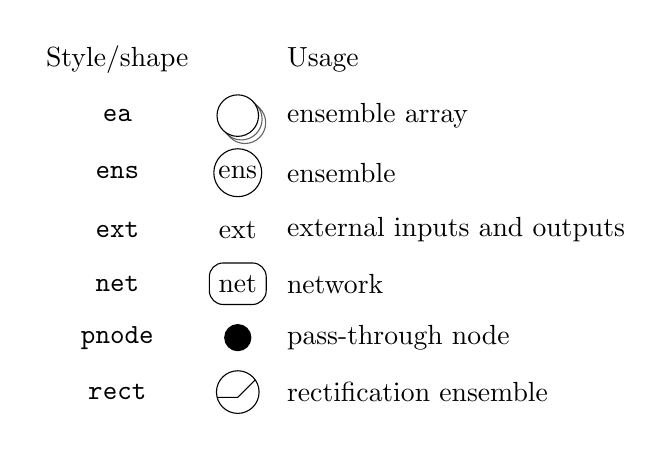
\begin{tikzpicture}
        \matrix [row sep=4pt, column sep=4pt] {
            \node {Style/shape}; & & \node [right] {Usage}; \\
            \node {\texttt{ea}}; & \node [nef,ea] {}; & \node [right] {ensemble array}; \\ 
            \node {\texttt{ens}}; & \node [nef,ens] {ens}; & \node [right] {ensemble}; \\ 
            \node {\texttt{ext}}; & \node [nef,ext] {ext}; & \node [right] {external inputs and outputs}; \\ 
            \node {\texttt{net}}; & \node [nef,net] {net}; & \node [right] {network}; \\ 
            \node {\texttt{pnode}}; & \node [nef,pnode] {}; & \node [right] {pass-through node}; \\
            \node {\texttt{rect}}; & \node [nef,rect] {}; & \node [right] {rectification ensemble}; \\ 
        };
    \end{tikzpicture}
    \caption{Node styles and shapes.}
\end{figure}

\paragraph{ea}
Use this style for ensemble arrays.

\paragraph{ens}
Use this style for single ensembles.

\paragraph{ext}
Use this style for inputs and outputs external to the displayed network.

\paragraph{net}
Use this style for networks.

\paragraph{pnode}
Use this style for pass-through nodes.

\paragraph{rect}
Use this style for rectification ensembles (i.e., all encoders are 1).

\subsection{Edge styles}
\begin{figure}
    \centering
    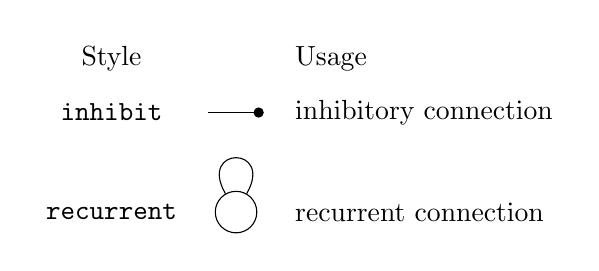
\begin{tikzpicture}
        \matrix [row sep=4pt, column sep=4pt] {
            \node {Style}; & & \node [right] {Usage}; \\
            \node {\texttt{inhibit}}; & \draw (-10pt, 0) -- (10pt, 0) [inhibit]; & \node [right] {inhibitory connection}; \\ 
            \node {\texttt{recurrent}}; & \node (ens) [nef,ens] {}; \path [nef] (ens) edge [nef,recurrent] (ens) ; & \node [right] {recurrent connection}; \\ 
        };
    \end{tikzpicture}
    \caption{Edge styles.}
\end{figure}

\paragraph{inhibit}
Use this style for inhibitory connections.

\paragraph{recurrent}
Use this style for recurrent connections. It will add a loop above an ensemble or network.


\section{Examples}

\subsection{Gated difference integrator (working memory)}
\begin{center}
    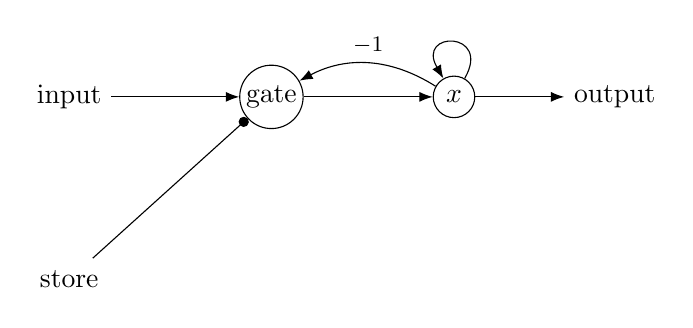
\begin{tikzpicture}[nef]
        \graph {
            input [ext] -> gate [ens] -> integrator/$x$ [ens] -> output [ext];
            integrator -> [bend right, "$-1$"] gate;
            integrator -> [recurrent] integrator;
            store -> [inhibit] gate;
        };
    \end{tikzpicture}
\end{center}

\begin{verbatim}
\usepackage{tikz}
\usetikzlibrary{graphs}
\usetikzlibrary{nef}
\usetikzlibrary{quotes}

%% ....

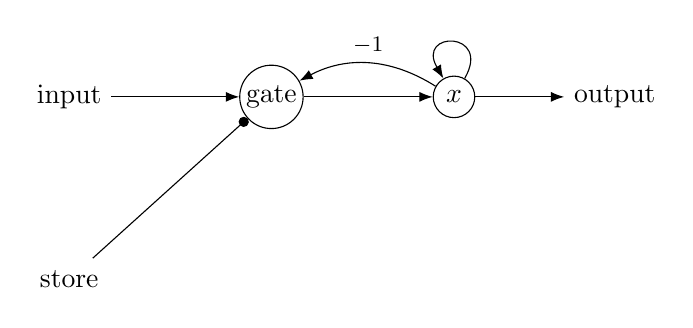
\begin{tikzpicture}[nef]
    \graph {
        input [ext] -> gate [ens] -> integrator/$x$ [ens] -> output [ext];
        integrator -> [bend right, "$-1$"] gate;
        integrator -> [recurrent] integrator;
        store -> [inhibit] gate;
    };
\end{tikzpicture}
\end{verbatim}


\printbibliography{}
\end{document}
